\section{Auswertung}
\subsection{Differenzen in Koinzidenzeinheiten}

Um zu verstehen, welchen Einfluss die Signallaufzeiten in der Schaltung haben,
wurde die Verzögerung dar Signale, die von den beiden zu SC2 gehörenden
Photomultipliern PM2 und PM4 ausgehen, mit einem Oszilloskop gemessen. Dabei
erhielten wir Bilder wie das in \fref{koinzidenz} dargestellte. 

\begin{figure}[htb]
   \centering
   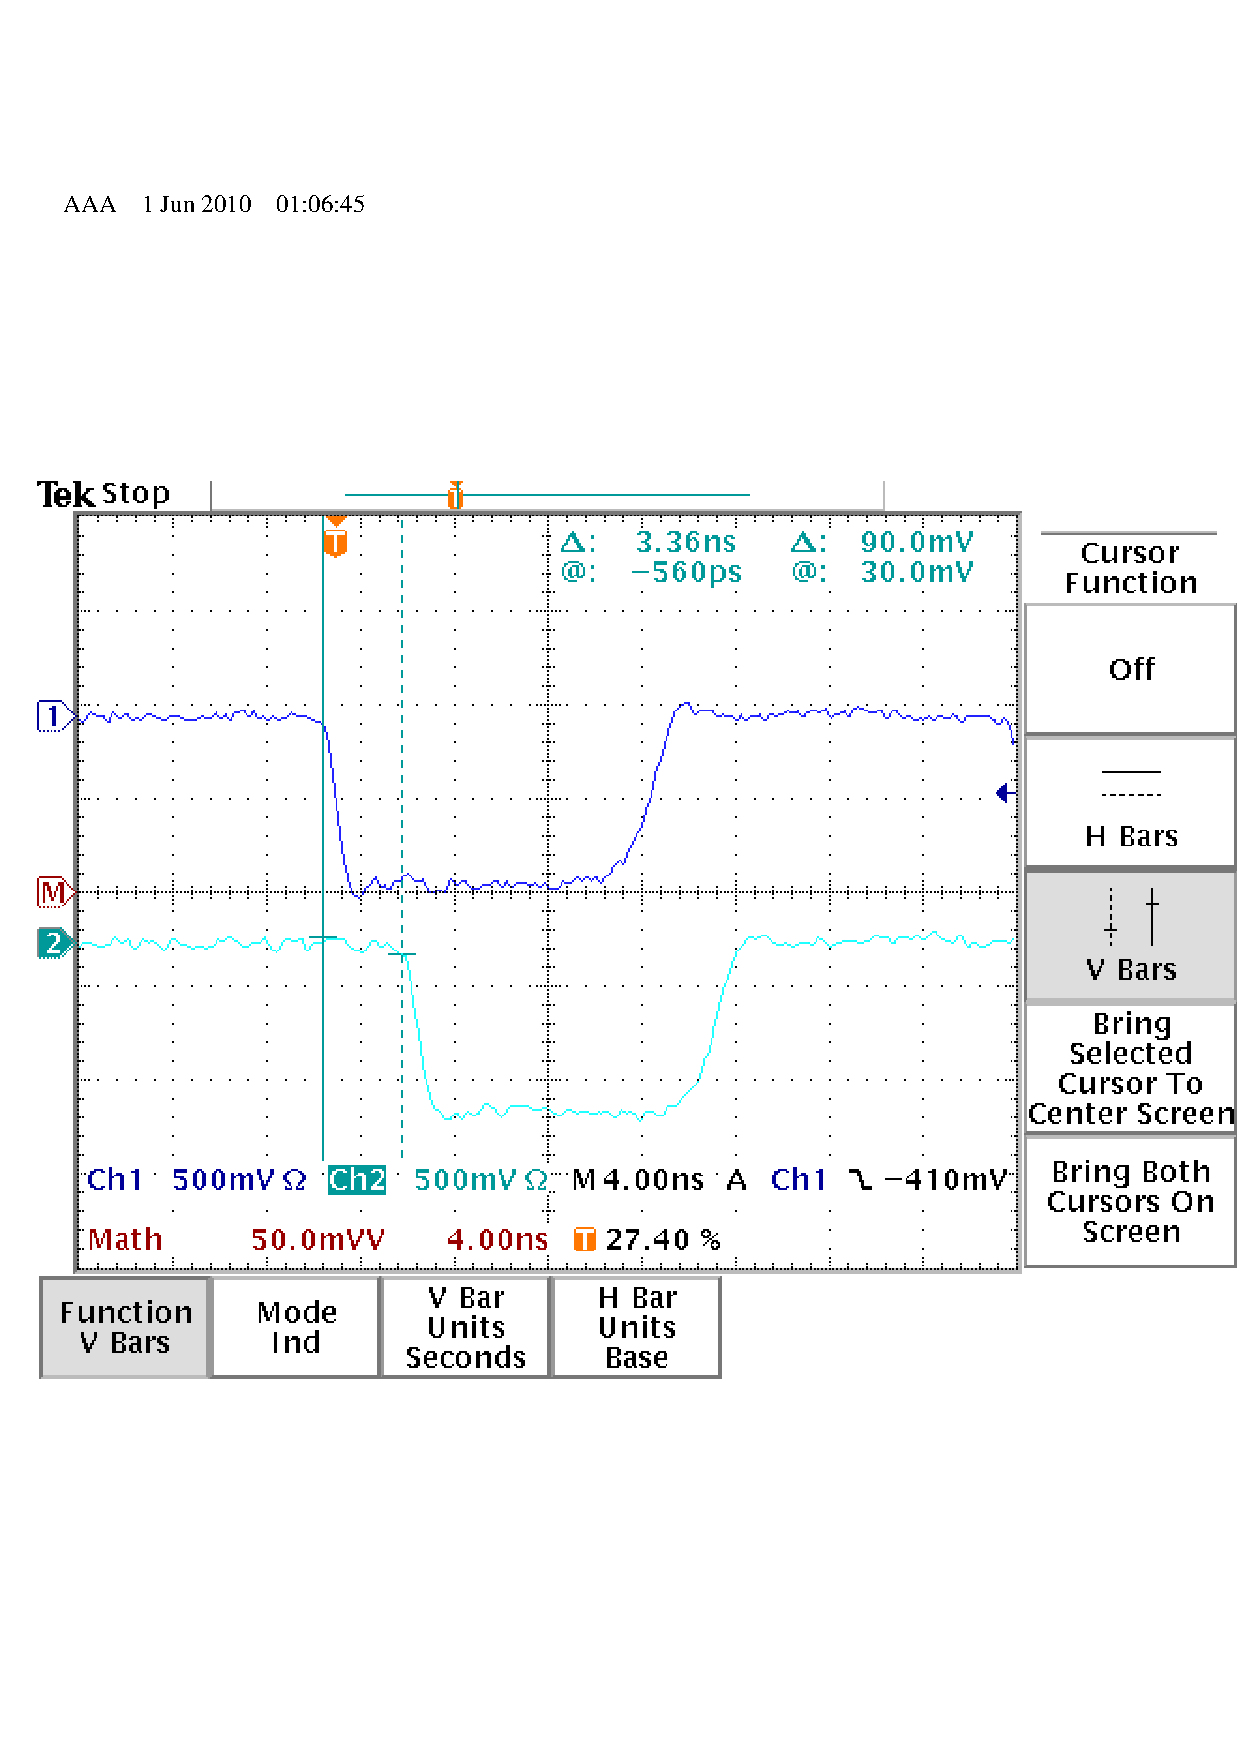
\includegraphics[width=1\columnwidth,keepaspectratio]{../data/TEK00010.pdf}
   \caption{Verzögerung in einer Koinzidenzeinheit}
   \label{fig:koinzidenz}
\end{figure}

Die Verzögerung wurde mit Hilfe der Positionsmarken, die zur Funktionalität des
Oszilloskops gehören, abgelesen, indem diese jeweils an den Beginn des Abfalls
der jeweiligen Kurve gefahren wurden. Die Differenz ist im oberen Bildteil in
der mit $\Delta:$ beginnenden Zeile abzulesen. Wir haben diese Messung sechs
mal durchgeführt. Die Zeitdifferenzen $t_i$ sind in \tref{diff} dargestellt.

\begin{table}[htbp]
\centering
% \setlength{\tabcolsep}{14pt}
\begin{tabular*}{0.95\columnwidth}{%
S[tabformat=1.2]%
S[tabformat=1.2]%
S[tabformat=1.2]%
S[tabformat=1.2]%
S[tabformat=1.2]%
S[tabformat=1.2]%
S[tabformat=2.1]%
}
\toprule
% daten aus ../data/TEK00006.pdf bis 12
{$t_1$} & {$t_2$} & {$t_3$} & {$t_4$} & {$t_5$} & {$t_6$} & {$t_7$}\\
\midrule
3,36 & 4,24 & 0,880 & 8,56 & 0,240 & 0,640 & 24,2\\
\bottomrule
\end{tabular*}
\caption{Messwerte der Verzögerungszeiten (angegeben in ns)}
\label{tab:diff}
\end{table}

Die Unsicherheiten der Zeiten liegen (je nach Messbereich) bei einem oder zwei
LSD (last significant digit). Wie man erkennen kann, schwanken die Zahlen
stark, was daran liegt, dass hier noch gar keine Ereignisselektion
stattgefunden hat und somit alle möglichen Events betrachtet wurden. Man kann
aber auch sehen, dass manche Zeitdifferenzen im Bereich von etwa
\SI{0,2}{\nano\second} liegen, also auf jeden Fall vernachlässigbar gegenüber
den Unsicherheiten der anderen Komponenten sind, zumal man davon ausgehen kann,
dass gerade diese Events diejenigen sind, die in Wirklichkeit gleichzeitig
stattfanden. Die Verzögerung wird also in diesem Bereich liegen und somit die
weitere Auswertung nicht beeinflussen.

\subsection{Bestimmung der Ereignisraten}

In diesem Versuchsteil wurden die Zählraten für verschiedene Kombinationen von
Photomultipliern und Szintillatoren gemessen.

\subsection{Ereignisraten für die einzelnen Photomultiplier}

Als erstes haben wir die in den einzelnen Photomultipliern auftretenden
Ereignisraten jeweils acht mal gemessen. Die resultierenden Mittelwerte der
Messwerte inkl. deren Fehler sind in \tref{pm_messwerte} zusammengetragen.

\begin{table}[htbp]
\centering
% \setlength{\tabcolsep}{14pt}
\begin{tabular*}{\columnwidth}{l|rrrrr}%
% S[tabformat=1.2]%
% S[tabformat=1.2]%
% S[tabformat=1.2]%
% S[tabformat=1.2]%
% S[tabformat=1.2]%
% S[tabformat=1.2]%
% }
\toprule
& {$PM_1$} & {$PM_2$} & {$PM_3$} & {$PM_4$} & {$PM_5$}\\
\midrule
Rate & 1094 & 1878 & 1936 & 1178 & 1797\\
Fehler & 33 & 43 & 44 & 34 & 42\\
\bottomrule
\end{tabular*}
\caption{Messwerte der Ereignisraten (in \SI{1}{\per\second}) in den
Photomultipliern $PM_i$}
\label{tab:pm_messwerte}
\end{table}
Hierbei wurde angenommen, dass man die statistischen Fehler über einfaches
Radizieren ermitteln kann:
\begin{equation}
σ = \Delta N = \sqrt{N},
\end{equation}
was nur bei hinreichend großen Messwertanzahlen $N$ korrekt ist. Da $N$ bei uns
in der Größenordnung von 1000 liegt, sollte diese Annahme gerechtfertigt sein.

Nun war zu untersuchen, wie stark die Effizienz abnimmt, wenn man in den
einzelnen Szintillationszählern eine Rechts-Links-Koinzidenz fordert. Dafür
haben wir eine entsprechende Logikschaltung aufgebaut, die diese zeitliche
Übereinstimmung überprüft. Auch hier haben wir immer acht mal gemessen; die
Mittelwerte sowie die Fehler können in \tref{SC2_SC3_koinzidenz} betrachtet
werden.

\begin{table}[htbp]
\centering
\begin{tabular*}{\columnwidth}{l|cc}
\toprule
& {SC2: $PM_2\wedge PM_4$} & SC3: $PM_3\wedge PM_5$\\
\midrule
Rate & 1094 & 1878\\
Fehler & 33 & 43\\
\bottomrule
\end{tabular*}
\caption{Messwerte der Ereignisraten (in \SI{1}{\per\second}) in den
Photomultipliern $PM_i$}
\label{tab:SC2_SC3_koinzidenz}
\end{table}